\chapter{La route Puno – Cusco}
\section*{22 mai 2015}
5 jours de vélo pour aller de Puno au bord du lac Titicaca à Cusco. \newline
 Un petit détour pour visiter le village de Lampa. \newline
 \newline
\centerline{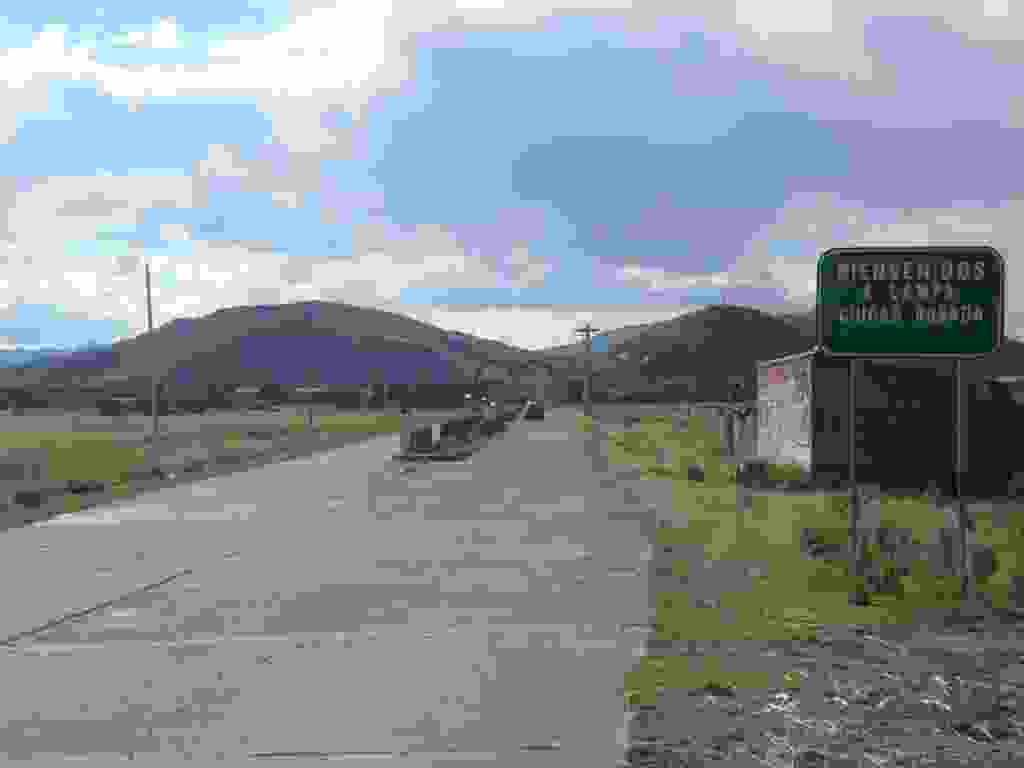
\includegraphics[width=\mywidth]{../wp-content/uploads/2015/05/P5124011-1024x768.jpg} } 
 \newline
 Très belle église, construite par les espagnols sur des fondations incas, comme beaucoup au Pérou. \newline
 \newline
\centerline{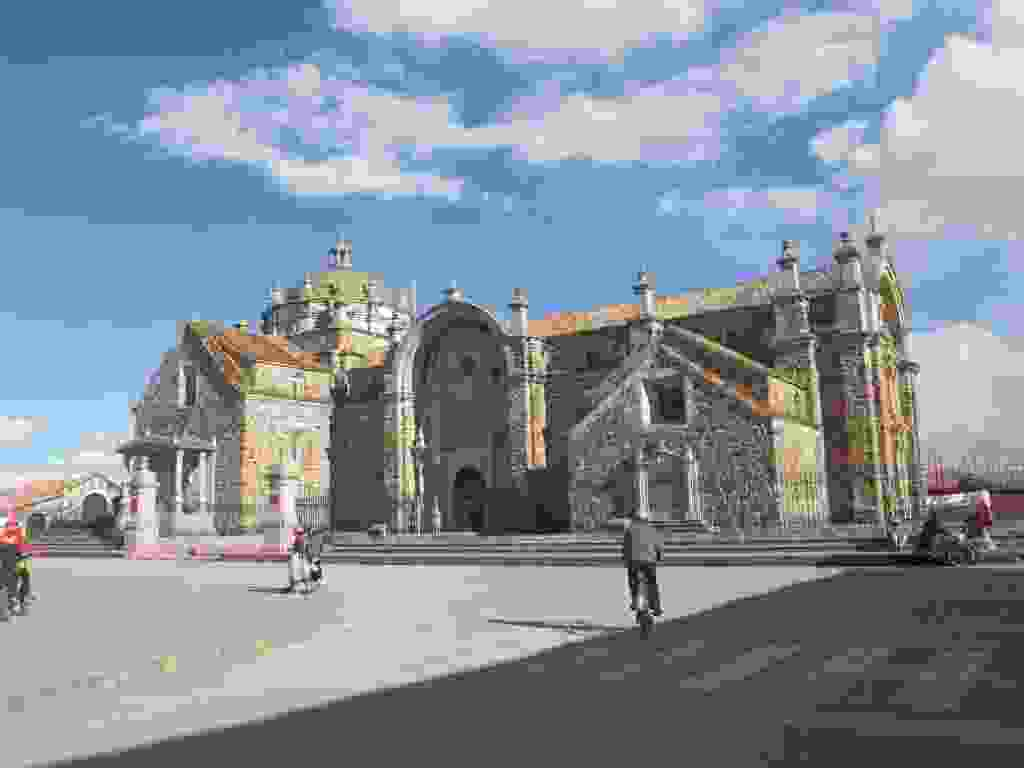
\includegraphics[width=\mywidth]{../wp-content/uploads/2015/05/P5124012-1024x768.jpg} } 
 \newline
 Les catacombes d´origine inca. \newline
 \newline
\centerline{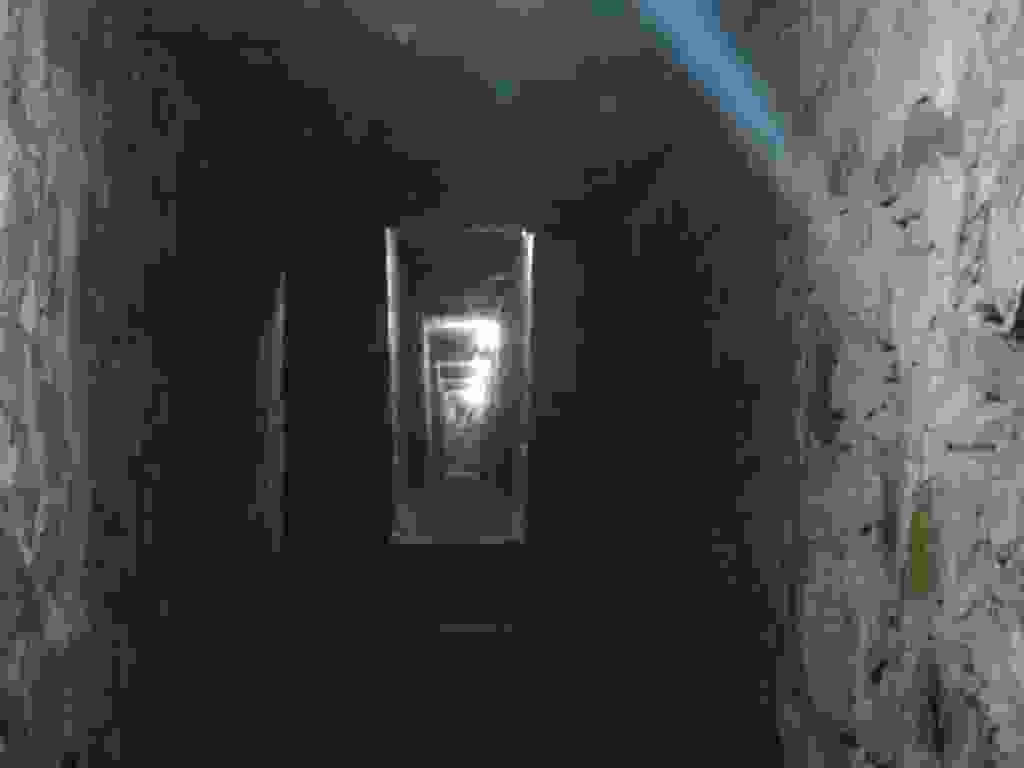
\includegraphics[width=\mywidth]{../wp-content/uploads/2015/05/P5124020-1024x768.jpg} } 
 \newline
 L´église contient une reproduction de la sculture La Pietà de Michel-Ange. \newline
 \newline
\centerline{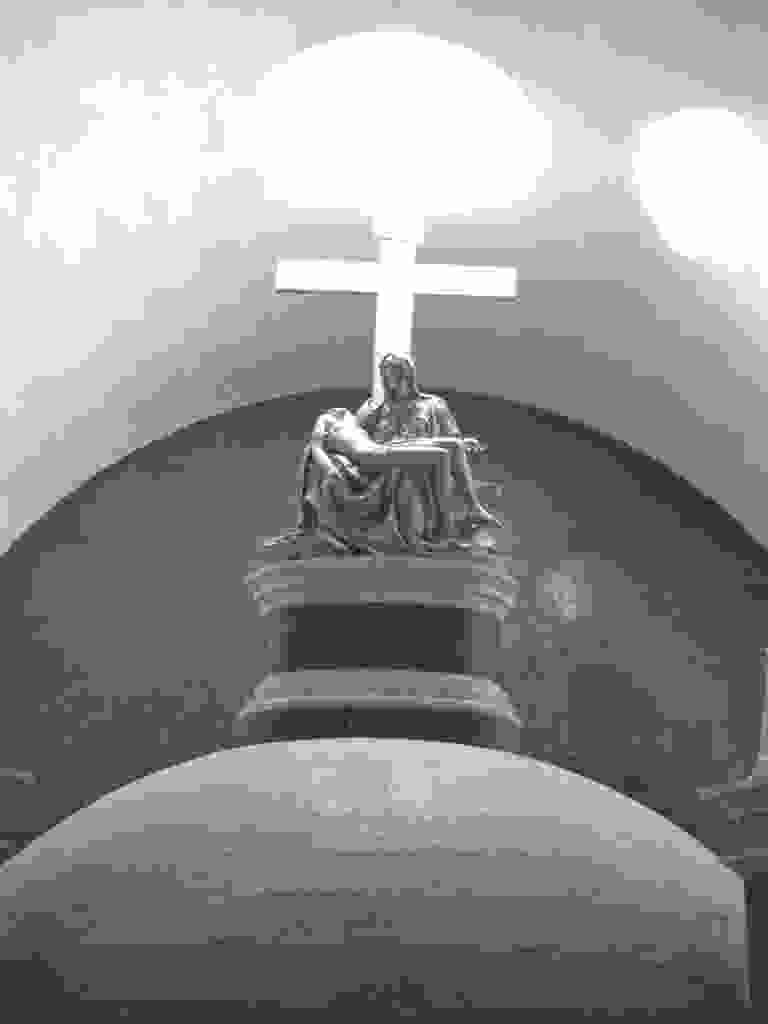
\includegraphics[width=\mywidth]{../wp-content/uploads/2015/05/P5124022-768x1024.jpg} } 
 \newline
 La route traverse de belles vallées et on aperçoit parfois des sommets enneigés. \newline
 \newline
\centerline{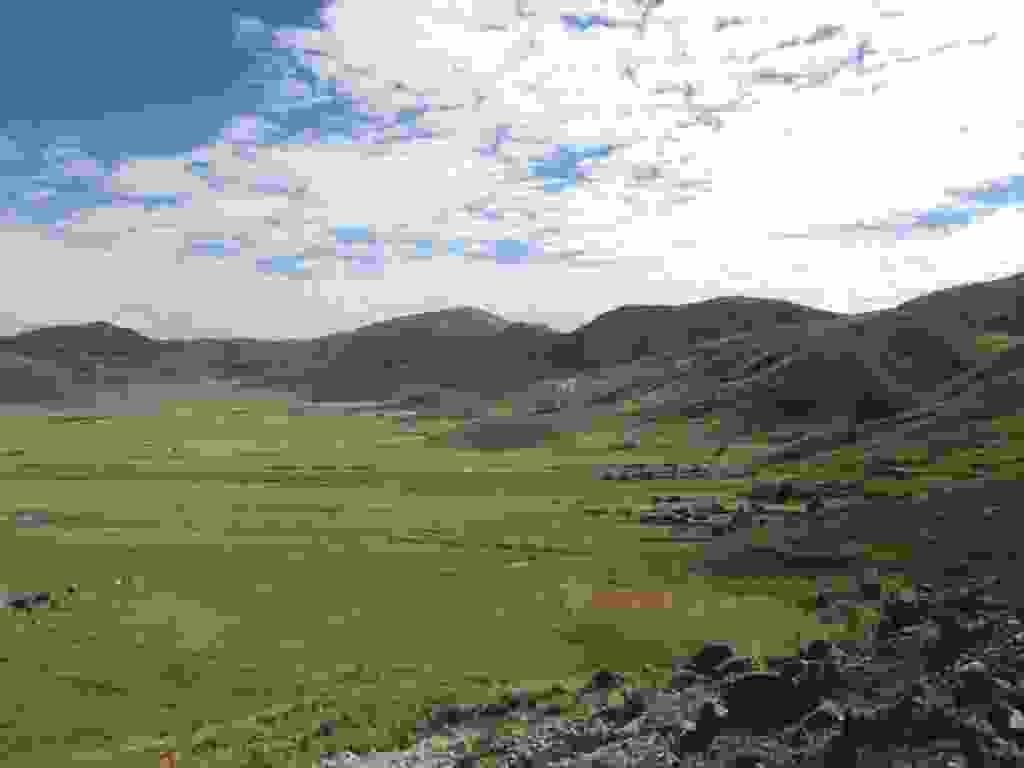
\includegraphics[width=\mywidth]{../wp-content/uploads/2015/05/P5134030-1024x768.jpg} } 
 \newline
 \newline
\centerline{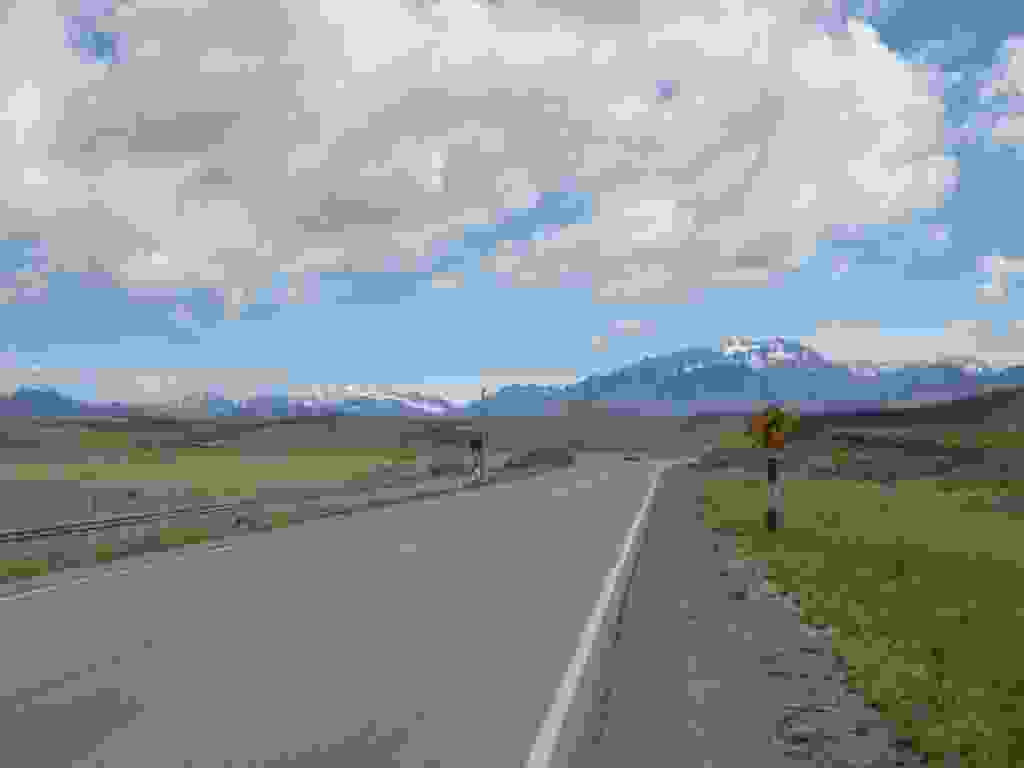
\includegraphics[width=\mywidth]{../wp-content/uploads/2015/05/P5144046-1024x768.jpg} } 
 \newline
 \newline
\centerline{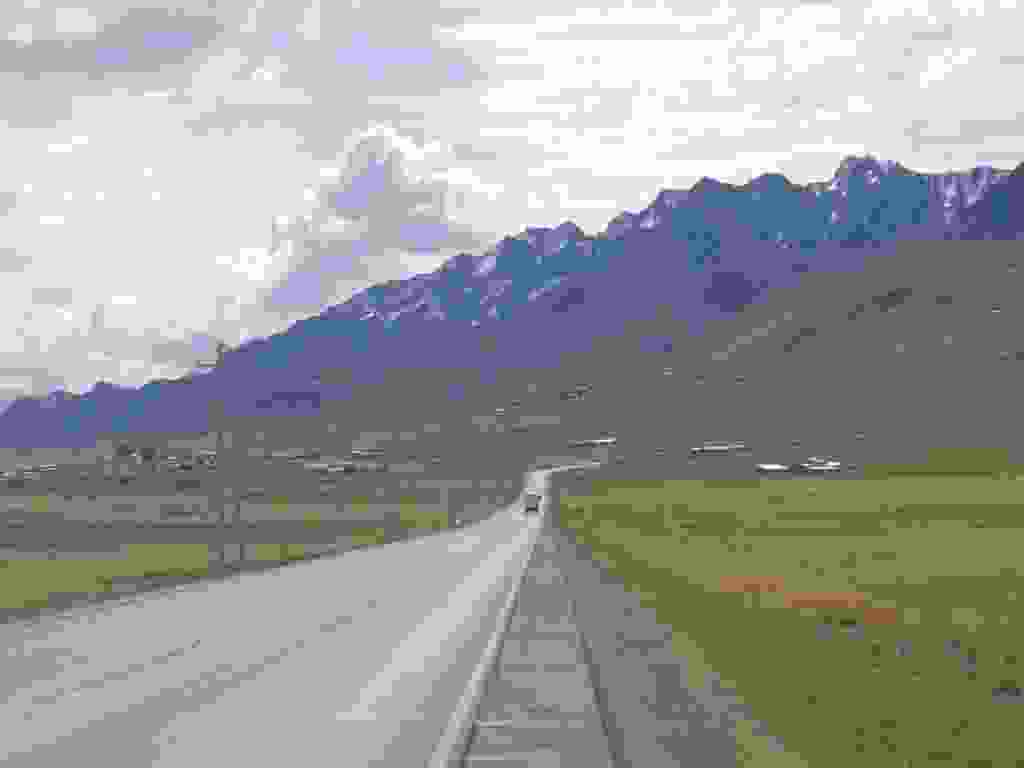
\includegraphics[width=\mywidth]{../wp-content/uploads/2015/05/P5144050-1024x768.jpg} } 
 \newline
 Le point le plus haut de la route : col de La Raya à 4300m. \newline
 \newline
\centerline{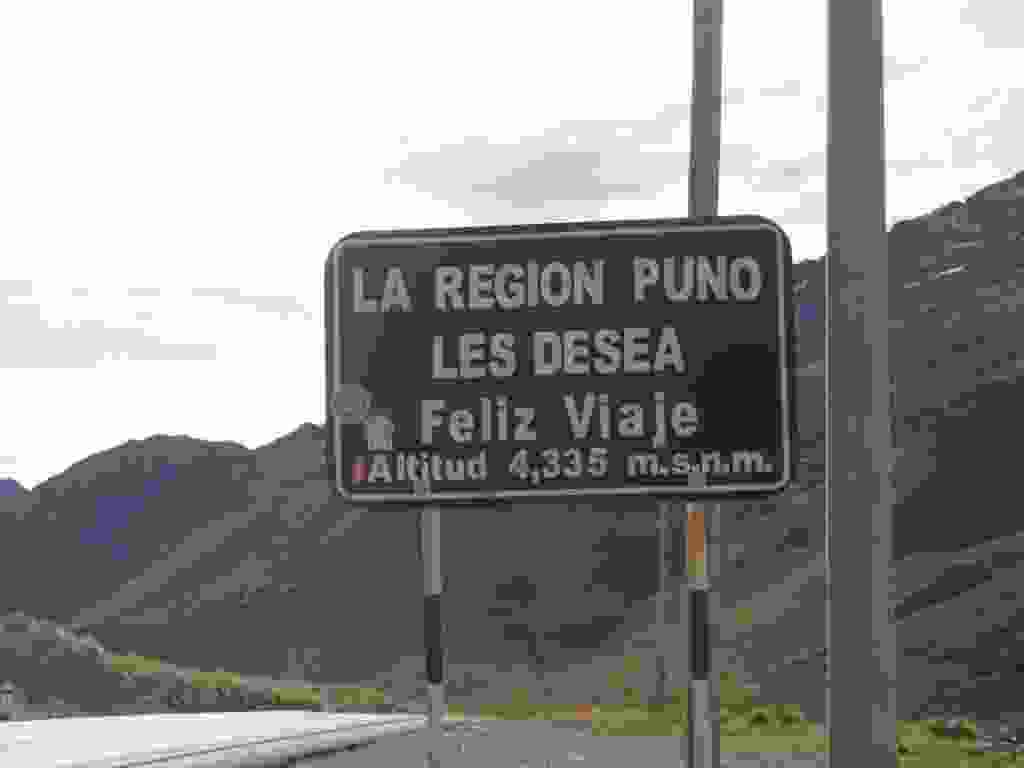
\includegraphics[width=\mywidth]{../wp-content/uploads/2015/05/P5144056-1024x768.jpg} } 
 \newline
 \newline
\centerline{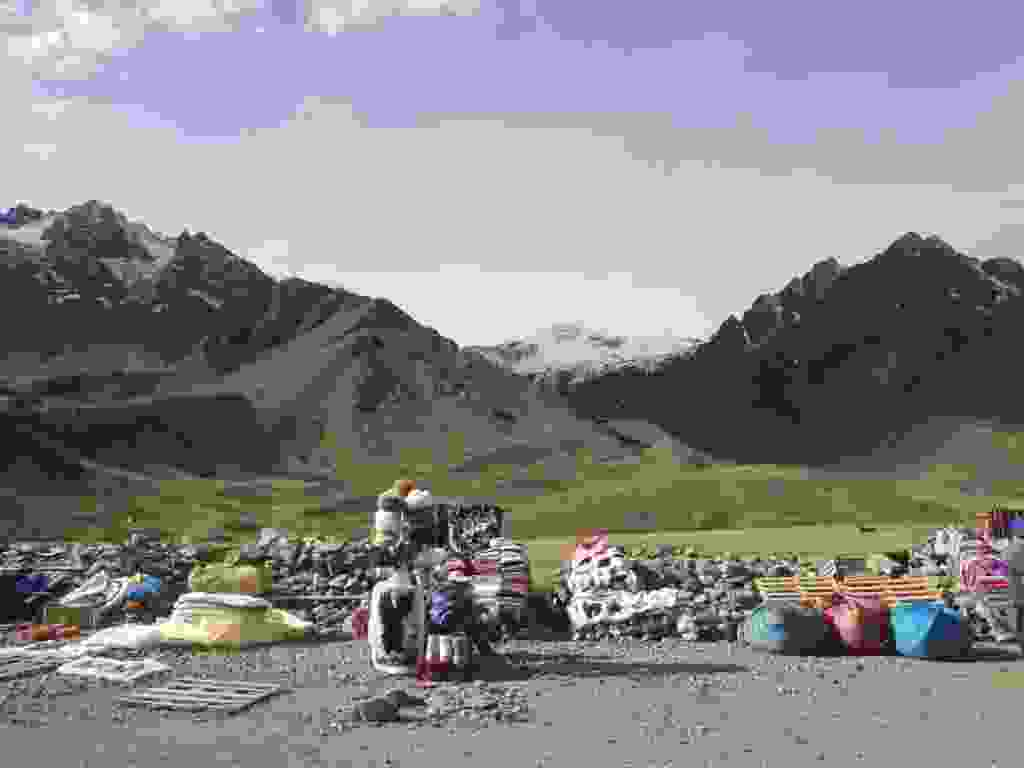
\includegraphics[width=\mywidth]{../wp-content/uploads/2015/05/P5144054-1024x768.jpg} } 
 \newline
 Bivouac dans la descente. \newline
 \newline
\centerline{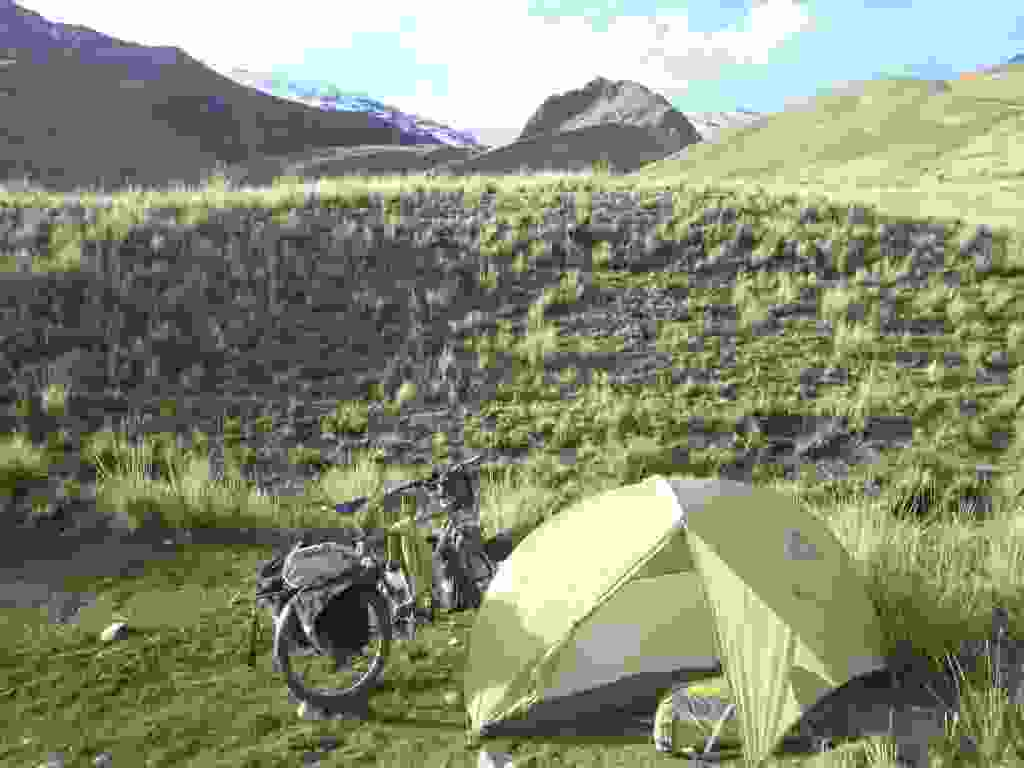
\includegraphics[width=\mywidth]{../wp-content/uploads/2015/05/P5144064-1024x768.jpg} } 
 \newline
 Le matin je me réveille avec un troupeau de lamas et alpagas juste au dessus de moi. \newline
 \newline
\centerline{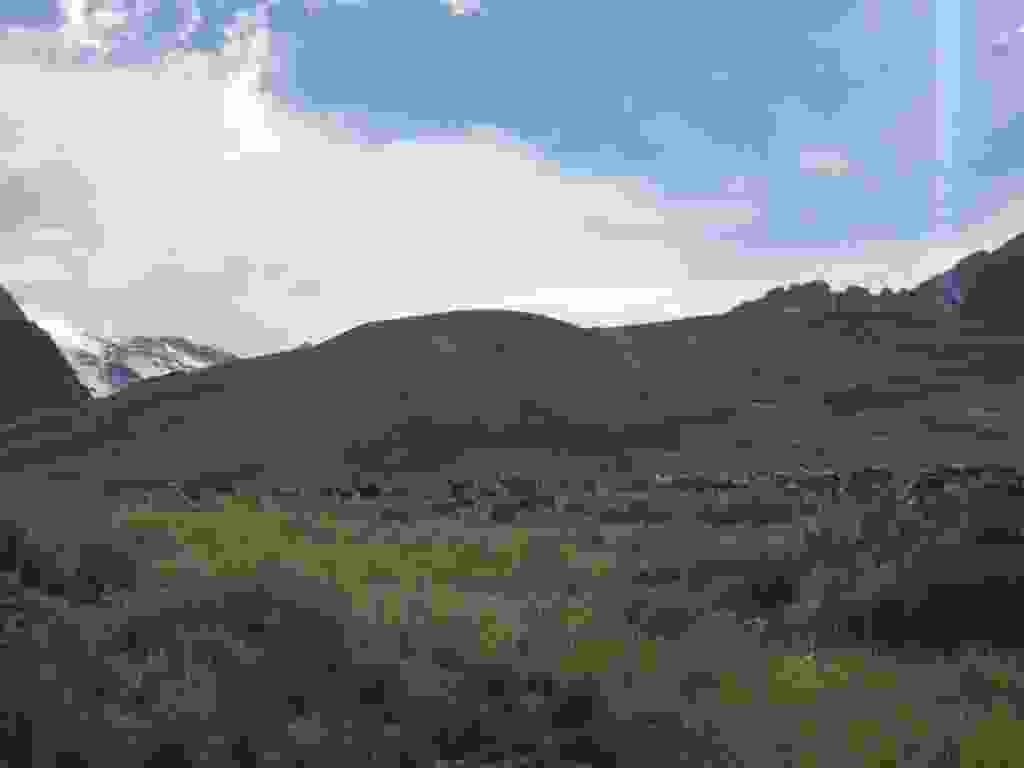
\includegraphics[width=\mywidth]{../wp-content/uploads/2015/05/P5154068-1024x768.jpg} } 
 \newline
 Sur la route beaucoup de petits restaurants où on peut manger un bon repas avec une soupe et un plat pour à peine 1,5€. \newline
 \newline
\centerline{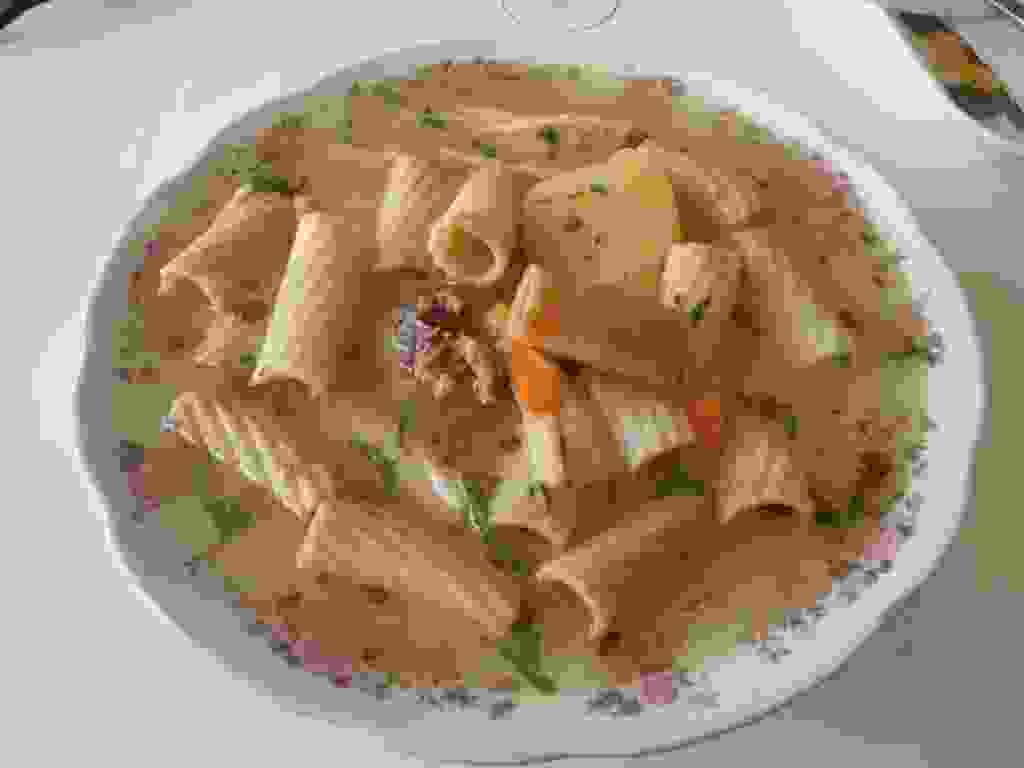
\includegraphics[width=\mywidth]{../wp-content/uploads/2015/05/P5134037-1024x768.jpg} } 
 \newline
 \newline
\centerline{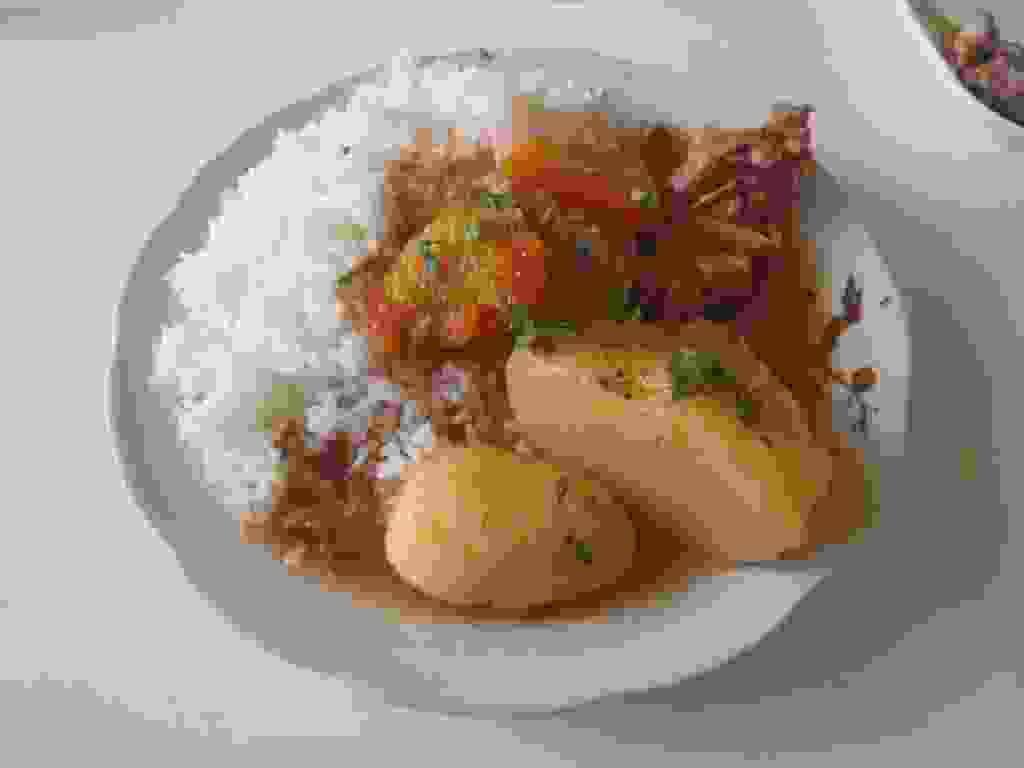
\includegraphics[width=\mywidth]{../wp-content/uploads/2015/05/P5134038-1024x768.jpg} } 
 \newline
 Avant d´arriver à Cusco, plusieurs sites archéologiques à visiter. \newline
 Le site de Rachqi, situé sur le chemin de l´inca, avec les restes d´un temple, d´habitations et de batiments de stockage de nourriture. \newline
 \newline
\centerline{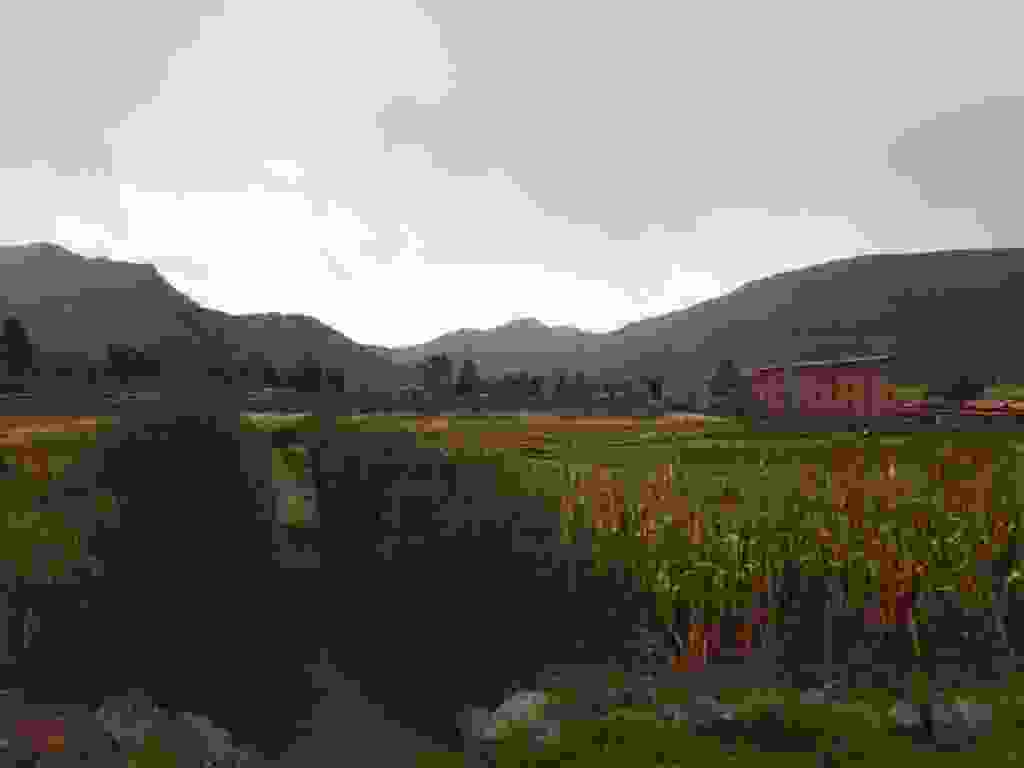
\includegraphics[width=\mywidth]{../wp-content/uploads/2015/05/P5154086-1024x768.jpg} } 
 \newline
 \newline
\centerline{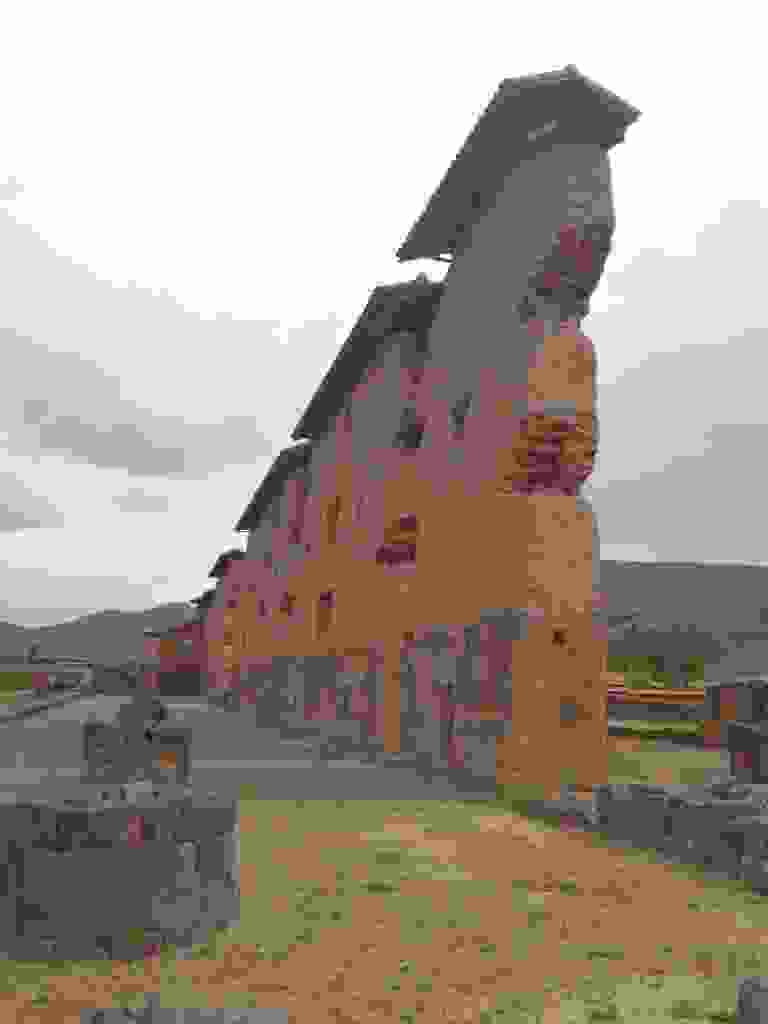
\includegraphics[width=\mywidth]{../wp-content/uploads/2015/05/P5154076-768x1024.jpg} } 
 \newline
 \newline
\centerline{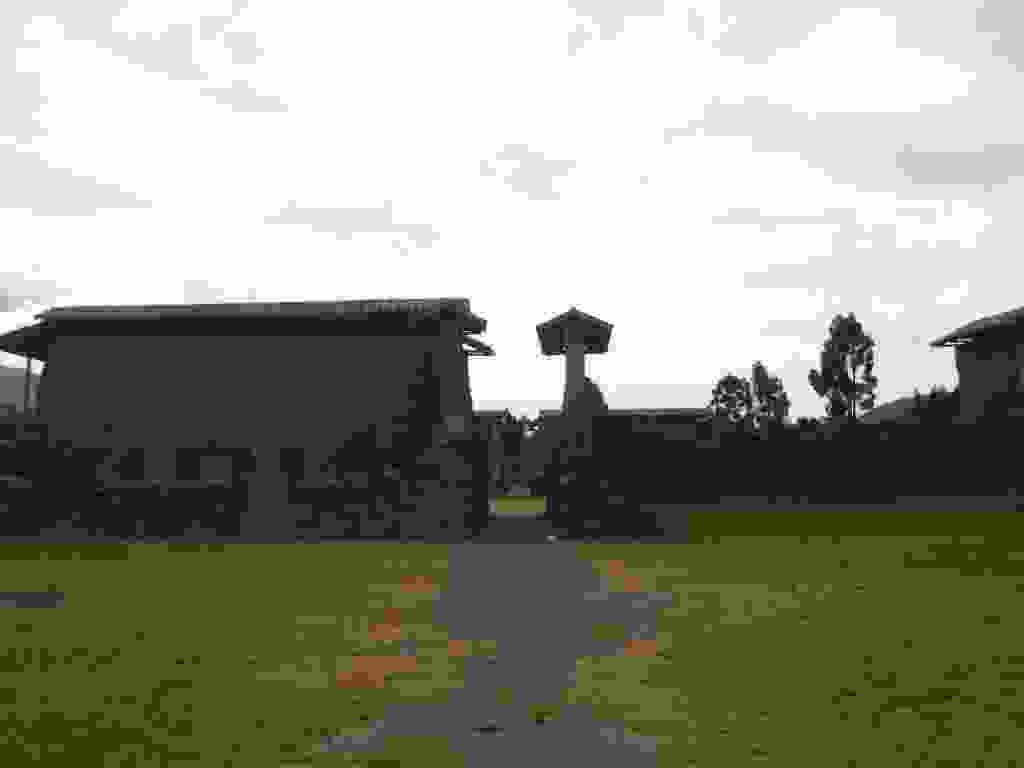
\includegraphics[width=\mywidth]{../wp-content/uploads/2015/05/P5154079-1024x768.jpg} } 
 \newline
 \newline
\centerline{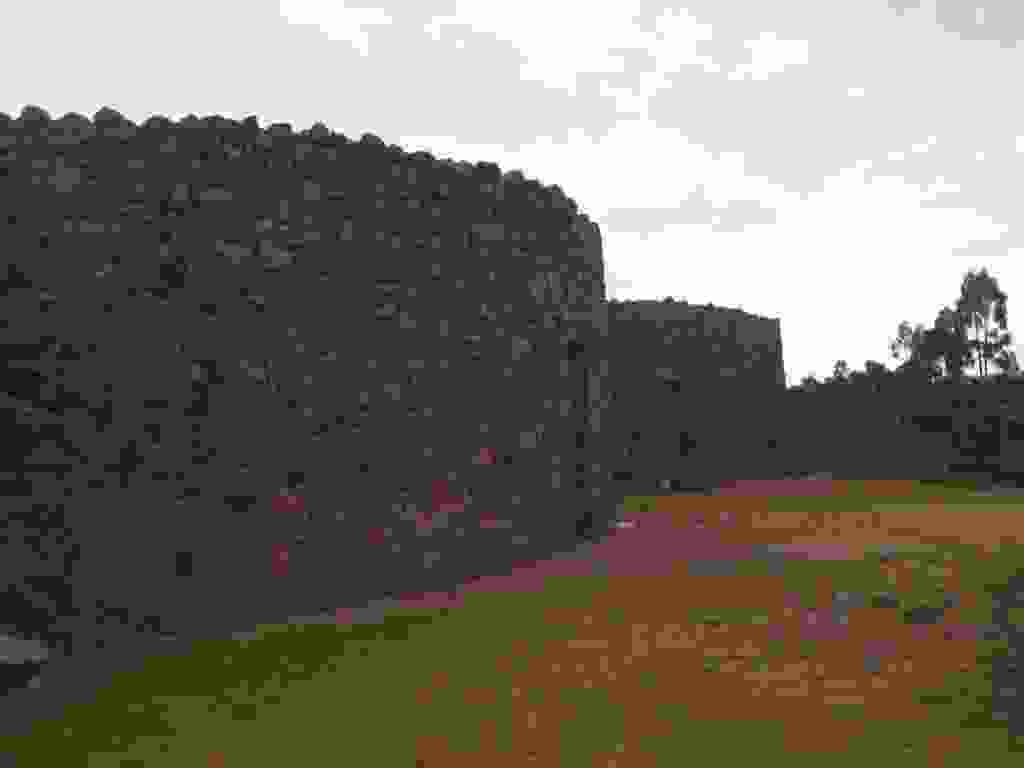
\includegraphics[width=\mywidth]{../wp-content/uploads/2015/05/P5154080-1024x768.jpg} } 
 \newline
 Dans le village d´Andihuaylillas, une belle église. \newline
 \newline
\centerline{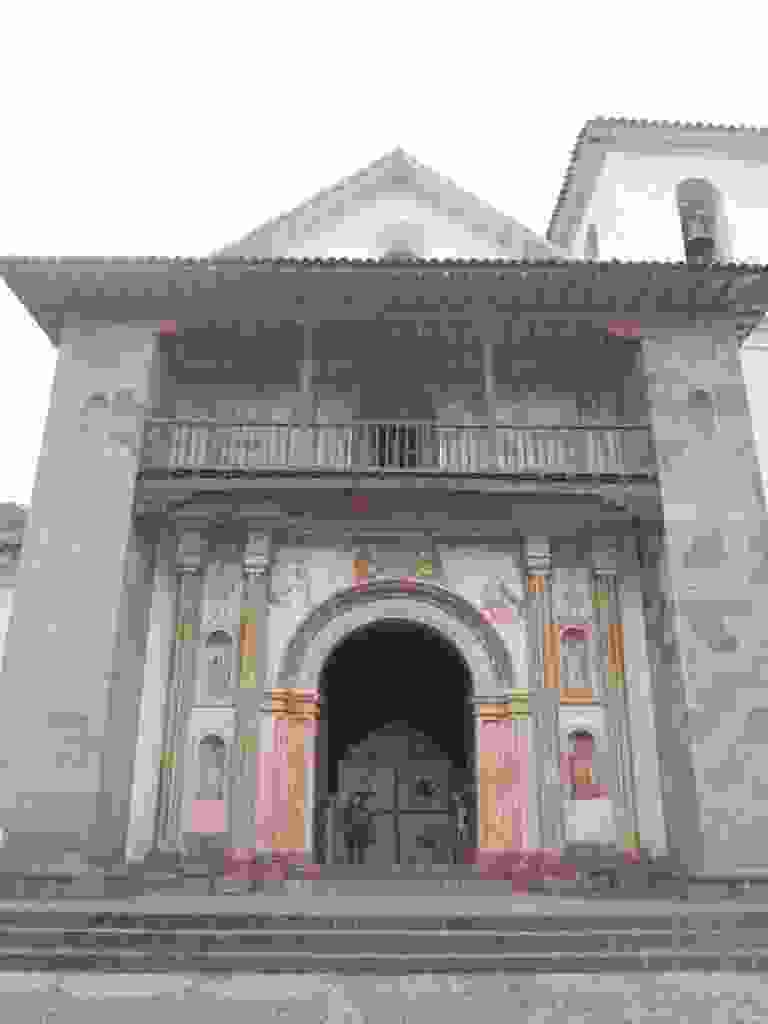
\includegraphics[width=\mywidth]{../wp-content/uploads/2015/05/P5164096-768x1024.jpg} } 
 \newline
 Au bord de la route une immense porte inca. \newline
 \newline
\centerline{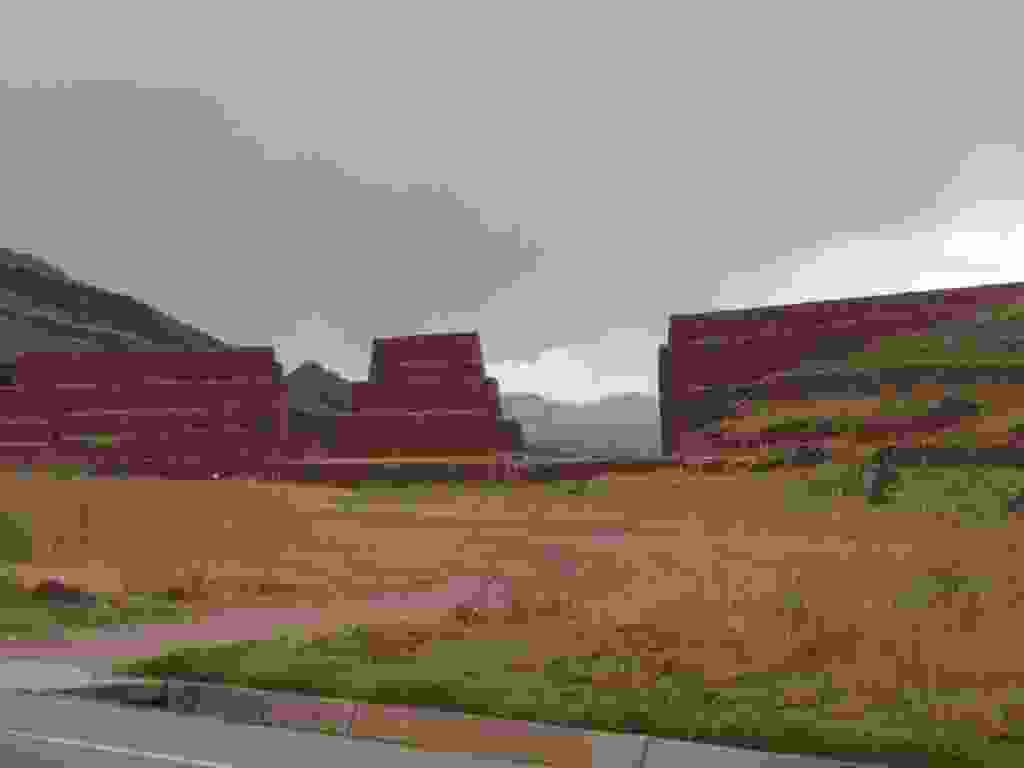
\includegraphics[width=\mywidth]{../wp-content/uploads/2015/05/P5164098-1024x768.jpg} } 
 \newline
 Puis le site pré-inca de Tiquillaka. \newline
 \newline
\centerline{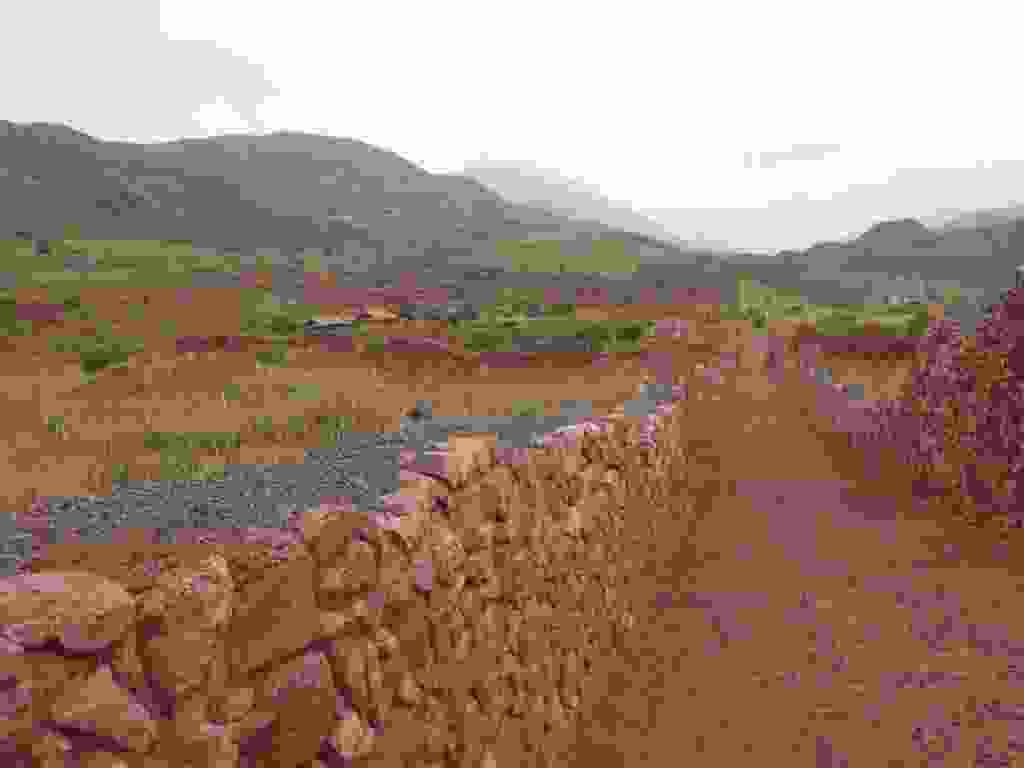
\includegraphics[width=\mywidth]{../wp-content/uploads/2015/05/P5164109-1024x768.jpg} } 
 \newline
 \newline
\centerline{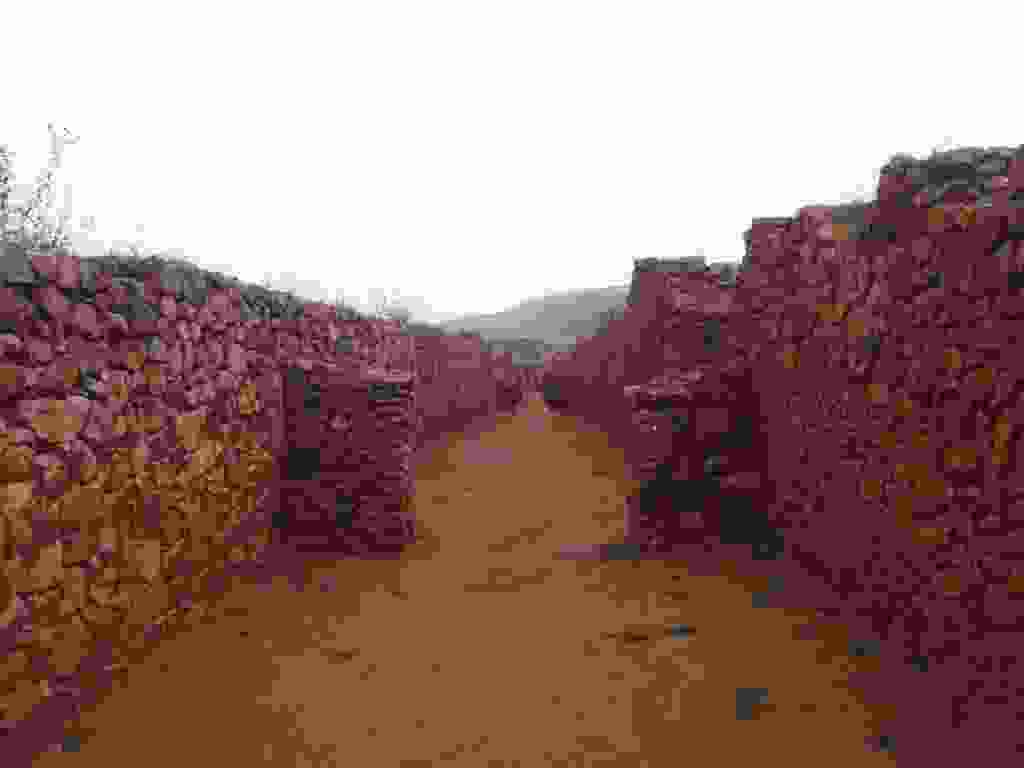
\includegraphics[width=\mywidth]{../wp-content/uploads/2015/05/P5164105-1024x768.jpg} } 
 \newline
 \newline
\centerline{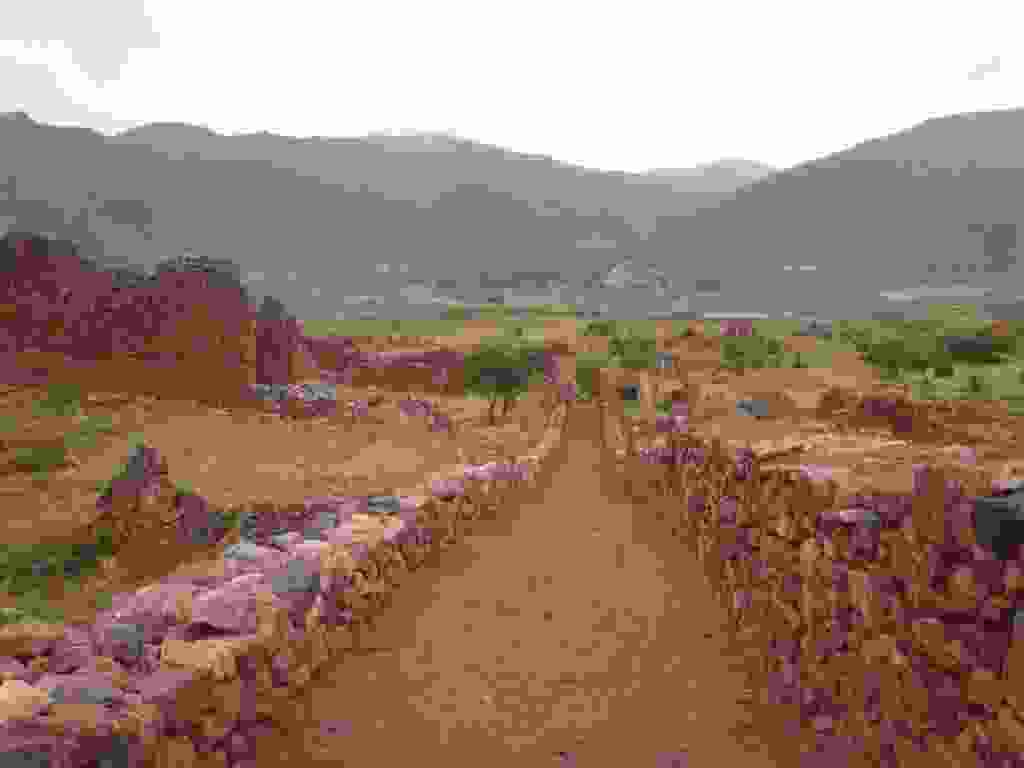
\includegraphics[width=\mywidth]{../wp-content/uploads/2015/05/P5164102-1024x768.jpg} } 
 \newline

\newpage
 
